\section{Method}
In this section the methodology is covered in four parts.
Firstly, the practical procedure chosen in this work for applying \spectral{} clustering  is given.
Secondly, choices and interpretations for the variable parameters in this algorithm are given.
Thirdly,  the datasets against which this will be measured are specified.
Fourthly, the procedure for checking IR safety is described.

    \begin{figure}[!t]
        \center
        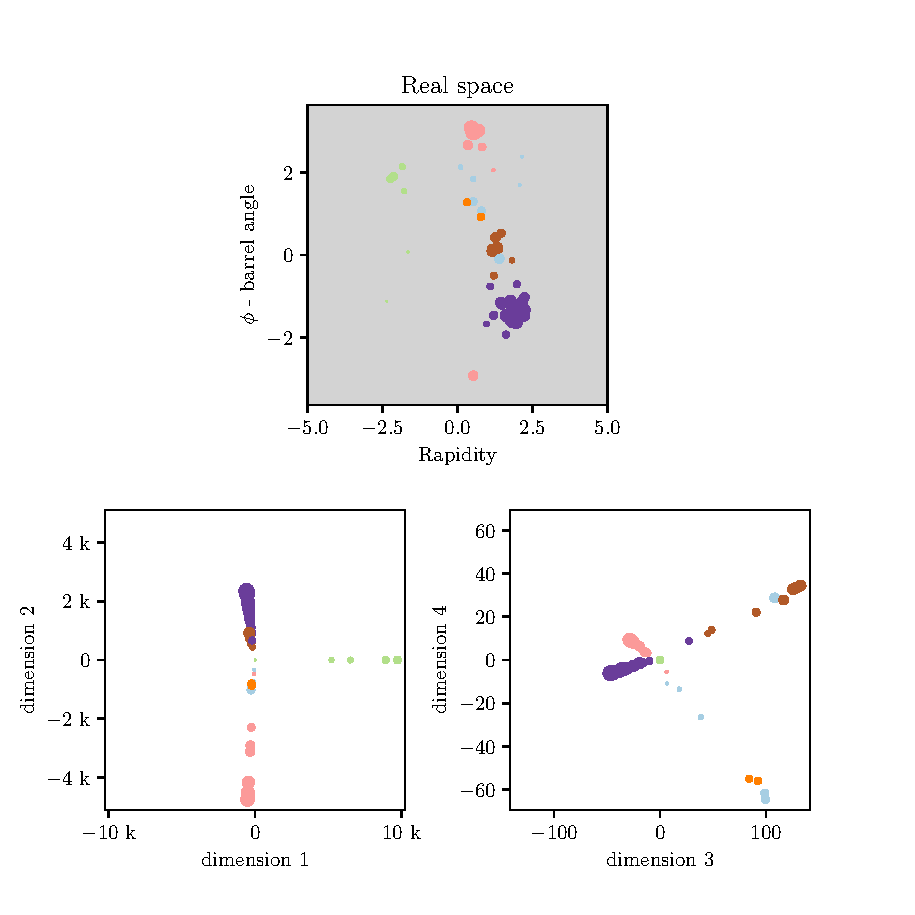
\includegraphics[width=0.7\textwidth]{graphics/embedding_space_simple2.pdf}
        \caption{A single event and its embedding space, as created by \spectral{} clustering.
            At the top the grey plot shows the particles in the event as points on the unrolled detector barrel.
            The colour of each point indicates the shower it came from.
            The lower two plots show the first 4 dimensions of the embedding space,
            and the location of the points within the embedding space.}\label{fig:embedding_space_simple}
    \end{figure}    


For clarity, note that the variable pseudorapidity is never used
in the algorithms proposed; all references to rapidity $y$ correspond to
\begin{equation}\label{eqn:rapidity}
    y = \frac{1}{2} \ln\frac{E + p_z}{E - p_z}.
\end{equation}

Besides rapidity, barrel angle, \(\phi\), is also used as a coordinate.
The barrel angle is the angle of the particle in the plane perpendicular to the beam.
Barrel angle and rapidity form an orthogonal coordinate system.

\subsection{Spectral clustering algorithm}\label{sec:spectralmethodalgo}
    For every simulated event the following process is used to identify the jets
   % should we point to the repo?
   % \footnote{Code available at \url{https://github.com/HenryDayHall/jetTools}}.
    To begin with, relevant cuts are applied to the particles to simulate the detector's
    reconstruction capability.
    (These are described in detail in section~\ref{sec:particle_data}.)
    Then all particles are declared pseudojets  and given an index, \(j = 1 \dots n\), with no particular order.
    The algorithm is agglomerative, recursively selecting pairs of pseudojets to merge;
    hence, the first iteration step is labelled \(t=1\).

    When the two pseudojets to be merged, \(i\) and \(j\), have been identified they are combined
    using the E-scheme.
    The E-scheme forms a new pseudojet by summing the \(4\)-momentum of the two join pseudojets;
    \(p(t+1)_l = p(t)_i + p(t)_j\).
    The steps used to select two pseudojets to merge proceed as follows;


    \begin{enumerate}
        \item \label{step:start} The pseudojets are used to form the nodes of a graph,
        the edges of which will be weighted by some measure of proximity between the particles called affinity.
        To obtain an affinity, first a distance is obtained.
        Between pseudojets \(i\) and \(j\) this would be \(d(t)_{i,j} = \sqrt{(y(t)_i - y(t)_j)^2 + (\phi(t)_i - \phi(t)_j)^2}\)
        where \(y(t)_j\) is the rapidity of pseudojet \(j\) at time step \(t\) and \(\phi(t)_j\) is the barrel angle, likewise for \(i\).
        No \(p_T\) dependence is used, as customary in many traditional jet clustering methods.

    \item \label{step:affinity} The affinity must increase as pseudojets become more similar,
        whereas the distance will shrink.
        We chose \(a(t)_{i,j} = \text{exp}(-d(t)_{i,j}^\alpha/\sigma_v)\),
        where $\alpha=2$ is the standard Gaussian kernel as
        used in~\cite{Belkin:2003_unfound4}.
            Distances much larger than \(\sigma_v\) are only allowed very small affinities,
            thus less influence over the clustering.

    \item\label{step:KNN} Pseudojets that are far apart have low affinity,
        hence are unlikely to be good candidates for combination.
        Removing these affinities reduces noise.
    A fixed number, \(k_\text{NN}\), of neighbours of each pseudojet is 
    preserved while all other affinities are set to zero.
    Thus, in a group with more than \(k_\text{NN}\) pseudojets,
    each pseudojet has at least \(k_\text{NN}\) non-zero affinities with other pseudojets.

\item\label{step:laplacean} These affinities allow the construction of the symmetric normalised
        Laplacian; which is proportional to \(-a(t)_{i, j}\)
        in the \(i\)$^{\rm th}$ row and \(j\)$^{\rm th}$ column and exactly \(1\) on the diagonal.
        For ease of notation, let \(z(t)_j\) be a measure of the size a pseudojet \(j\) contributes to a cluster,
        with \(z(1)_j = \sum_k a_{i,k}\).
        Then define square matrices \(A(t)_{i, j} = (1 - \delta_{i, j}) a(t)_{i, j}\) and \(Z(t)_{i, j} = \delta_{i, j} z(t)_i\)
        The Laplacian can now be written as
       \begin{equation}\label{eqn:Laplacian}
        L(t) = Z(t)^{-\frac{1}{2}}(Z - A)Z(t)^{-\frac{1}{2}}
       \end{equation}
        After each step this Laplacian shrinks by one row and column.
        When two pseudojets have been combined, instead of calculating \(z_j\) as the sum of the affinities of the combined pseudojet,
        the new \(z_j\) is the sum of the two previous \(z_j\)'s.
        For example, if pseudojets \(1\) and \(2\) from \(t=1\) are to be combined to make pseudojet \(1\) in \(t=2\),
        then \(z(2)_{1} = z(1)_1 + z(1)_2\) rather than the sum of affinities between the new pseudojet \(1\) and other pseudojets in step \(t=2\).
        This condition is seen to be required for IR safety. 

        As such, after the first time step, \(L\) will no longer be a proper graph Laplacian.
        Its rows and columns do not sum to zero.
        However, this new \(L\) appears to maintains similar behaviour
        to a propper Laplacian in the embedding space it creates.

    \item \label{step:eigenvectors} The eigenvectors of $L(t)$, ($q$ the eigenvalue index)
            \begin{equation}
                L(t) h(t)_q = \lambda(t)_q h(t)_q,  \; q=1, \ldots, c
            \end{equation}
            	are used to create the embedding of the pseudojets.
            The eigenvector corrisponding to the smallest eigenvalue represents the trivial solution,
            that places all points in the same cluster (see Sec.~\ref{sec:spectral_theory}).
            All non-trivial eigenvectors, corresponding
            to eigenvalues less that an eigenvalue limit \(\lambda(t)_c < \lambda_\text{limit} < \lambda(t)_{c+1}\)
            are retained. See section~\ref{sec:eig_norm}.
            {NOTE: Eigenvalues $0\leq \lambda(1)\leq 2$.
            However, $\lambda(t)$ for $t>1$ are bounded but in a different range.} 

        \item \label{step:compression} A eigenvector is divided by the corresponding eigenvalue raised to \(\beta\).
            This acts to compress the dimensions that hold less information, again, see section~\ref{sec:eig_norm}.
            The embedding space can now be formed.
            The eigenvectors have as many elements as there are pseudojets and the coordinates of
            the \(j^\text{th}\) pseudojet at time step \(t\)
            are defined to be
            \(m(t)_j = \left(\lambda_1(t)^{-\beta} h_1(t)_j, \dots \lambda_c(t)^{-\beta} h_c(t)_j\right)\).
            %The first embedding space of a clustering is shown in Fig.~\ref{fig:embedding_space_simple}.

        \item  A measure of distance between all pseudojets in the embedding space is calculated.
            In the embedding space angular distances are most appropriate (see section~\ref{sec:embedding_distance}):
            \begin{equation}
                d'(t)_{i, j} = \arccos\left|\frac{m(t)_i\cdot m(t)_j}{\|m(t)_i\| \|m(t)_j\|}\right|.
            \end{equation}
            where \(\|m\|\) is the (Euclidean) length of \(m\).

        \item\label{step:stoppingcondition}

            Provided the mean of this distance is less than \stoppingdeltar{}, that is,
            \begin{equation}
                \frac{2}{c(c-1)}\sum_{i\ne j} d'(t)_{i, j} < \stoppingdeltar{},
            \end{equation}
            then the two pseudojets that have the smallest embedding distance are combined.
            NOTE: there are $\frac{c(c-1)}{2}$ possible pairs, 
            where \(c\) is the number of pseudojets remaining.
            (Reasons for this stopping condition are given in section~\ref{sec:stopping_condintion}.)
        
     \end{enumerate}
    %  
    When the mean of the distances in the embedding space rises above \stoppingdeltar{},
    then all remaining pseudojets are promoted to jets.
    Jets with less than 2 tracks are removed and their contents considered noise.
    Further cuts may then be applied as described in section~\ref{sec:particle_data}.

    These steps will form a variable number of jets from a variable number of particles.
    An example of the constructed first embedding space is shown in Fig.~\ref{fig:embedding_space_simple}.
    This illustrates how the embedding space highlights the clusters.

\subsection{Tunable parameters}\label{sec:spectralmethodparam}
Unlike most Machine Learning (ML) techniques, \spectral{} clustering does not have large arrays of learnt parameters.
The parameters for the clustering are a small, interpretable  set.
Appropriate values were chosen by performing scans and observing the influence of changes to the parameters on jets formed.

In section~\ref{sec:spectralmethodalgo}, 6 parameters are named:
\(\sigma_v\), \(\alpha\), \(k_\text{NN}\), \(\lambda_\text{limit}\), \(\beta\) and \stoppingdeltar{}.
These parameters have a range of values for which sensible results are obtained.
The interpretation of these parameters is as follows.
\begin{itemize}
    \item \(\sigma_v\): introduced in step~\ref{step:affinity}, this is a scale parameter in physical space.
                      The value indicates an approximate average distance for particles in the same shower,
                      or alternatively, the size of the neighbourhood of each particle.
                      It is closely tied to the stopping parameter for the \genkt{} algorithm,
                      \ktstoppingdeltar{},
                      they both relate to the width of the jets formed.
                      It should take values on the same order of magnitude as \ktstoppingdeltar{},
                      \sout{, i.e.,  of \(\mathcal{O} (0.1)\)}.
    \item  \(\alpha\): also introduced in step~\ref{step:affinity},
           this changes the shape of the distribution used to describe the neighbourhood of a particle.
           Higher values reduces the probability of joining particles outside \(\sigma_v\);
           \(\alpha=2\) defines a Gaussian kernel.
       \item \(k_\text{NN}\): introduced in step~\ref{step:KNN}, this dictates the minimum number of non-zero affinities around each point.
           Lower values create a sparser affinity matrix, reducing noise at the potential cost of lost signal.
           Values above \(7\) are seen to have little impact.
       \item  \(\lambda_\text{limit}\): introduced in step~\ref{step:eigenvectors}, is a means of limiting the number of eigenvectors used
           to create dimensions in the embedding space.
           Only eigenvectors corresponding to eigenvalues less than \(\lambda_\text{limit}\) are used.
           Thus, the number of dimensions in the embedding space can be increased with a larger \(\lambda_\text{limit}\). 
           However, as the eigenvalues will be influenced by the number of clear clusters available, 
           there will not be the same number of dimensions in each event.
           (This is discussed in section~\ref{sec:eig_norm}.)
           For a symmetric Laplacian the eigenvalues are \(0 \leq \lambda_1 \leq \lambda_2 \leq \cdots \lambda_n \leq 2\),
           and \(\lambda_k\) is related to the quality of forming \(k\)
           clusters \cite{JamesRLee:2014_unfound736},
           so values of $\lambda_{\mathrm limit} < 1$ are sensible choices.
       \item  \(\beta\): introduced in step~\ref{step:compression}, it 
          accounts for variable quality of information in the eigenvectors, as given by their eigenvalues,
        in such a way that the dimensions of the embedding spaces 
        corresponding to higher eigenvalues are compressed.
        in such a way that the dimensions of the embedding spaces with lower
        quality information are compressed.
        The larger the value of \(\beta\) the more dimensions with
        lower quality information are compressed.
        (This is discussed in section~\ref{sec:eig_norm}.)
%        This is should be \(\mathcal{O}(1)\).
    \item \stoppingdeltar{}: is introduced in step~\ref{step:stoppingcondition}, it
         determines the expected spacing between jets in the embedding space.
         As the number of dimensions in the embedding space grows with increasing 
         number of clear clusters, it will not result in the same or
         similar number of clusters each time.

\end{itemize}


To investigate the behaviour of the clustering when the parameters change, scans where performed.
On a small sample of 2000 events  the clustering is performed with many different parameter choices.

With the aid of MC truth information a metric of success can be created.
For each object we wish to find (e.g., a \bthing{quark}) 
the MC truth can reveal which of the particles that are visible to the detector have
been created by that object.
In many cases, a particle seen in the detector will have been created by two objects,
such as a particle coming from an interaction between a \(b\bar{b}\) pair,
in these cases both objects are considered together.
The complete set of visible particles that came from these objects could be referred to as their descendants.
The aim in jet clustering is to capture only all of the descendants in the same number of jets as there were objects that created them.
So the descendants of a \(b\bar{b}\) pair should be captured in exactly 2 jets.

    \begin{figure}[!t]
        \begin{minipage}[c]{0.6\textwidth}
            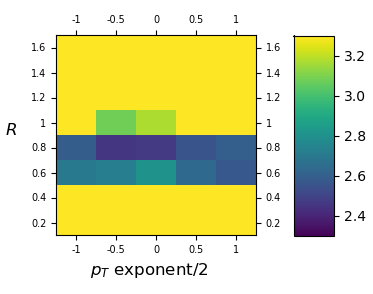
\includegraphics[width=1\textwidth]{graphics/trangle_scan_genkt}
        \end{minipage}\hfill
        \begin{minipage}[c]{0.35\textwidth}
            \caption{The \genkt{} algorithm has 2 parameters that can be varied.
                The stopping condition, \ktstoppingdeltar{}, and a multiple for the exponent of the \(p_T\) factor.
                When the exponent of the \(p_T\) factor is \(-1\) the algorithm becomes the \antikt{} algorithm.
                Here, the ``Loss'', as described in Eq.~(\ref{eqn:loss}), is shown as a colour gauge for a number of parameter combinations.
             }\label{fig:scan_genkt}
        \end{minipage}
    \end{figure}    

There are two ways a jet finding algorithm can make mistakes in this task:
the first is to omit some of the descendants of the objects being reconstructed, causing the jet to have less mass than it should;
the second is to include particles that are not in the descendants of the objects being reconstructed, such as initial state radiation or particles from other objects,
causing the jet to have more mass than it should.
The effects of these mistakes will cancel in the jet mass,
but they are both still individually undesirable,
so separate metrics are made for each of them.
The first is ``signal mass lost", the difference between the mass of the jets and the mass they would have had if all they contained all descendants of the object being reconstructed.
The second is ``background contamination", the difference between the mass of jets and the mass they would have if they did not contain anything but descendants of the objects being reconstructed.
A loss function is constructed as a weighted euclidean combination of these two;
\begin{equation}\label{eqn:loss}
\text{Loss} = \sqrt{w\,(\text{Background contamination})^2 + (\text{Signal mass lost})^2}.
\end{equation}
Where \(w\) is a weighting used to alter the preference for suppressing signal mass lost verses reducing background contamination.
When applying an \antikt{} algorithm, increasing \ktstoppingdeltar{} will result in lower signal mass loss, in exchange for a higher background contamination.
The standard choice for this process is \(\ktstoppingdeltar{}=0.8\).
This value of \ktstoppingdeltar{} slightly prefers suppressing signal mass lost over background contamination,
to create the clearest mass peaks.
To make the loss reflect this we chose \(w = 0.73\).

An example of this scan for the \genkt{} algorithm is given in Fig.~\ref{fig:scan_genkt}. 
It can be seen that, while good results are possible with many values of the \(p_T\) exponent,
                \ktstoppingdeltar{} must fall in a narrow range. We thus deem this choice of  stopping condition, \(\stoppingdeltar{}_{k_T}=0.8\), to be rather fine-tuned.

For \spectral{} clustering there are more than 2 variables to deal with, 
so a set of two dimensional slices are extracted. 
These slices have been chosen to include the best performing combination.
%
    As can be seen in Fig.~\ref{fig:scan_spectral}, the parameters choices  are not fine-tuned. That is, 
    unlike the \antikt{} algorithm, there is flexibility in all parameter choices. For example, it can be seen that some parameters, such as \(\alpha\), \(k_\text{NN}\), \(\beta\)
    and \(\lambda_\text{limit}\) are relatively unconstrained,
    yielding  good results for a wide range of values.
    Even when \stoppingdeltar{} and, especially, \(\sigma_v\) yield some large signal losses,
    say, for \(R=1.22\) or \(1.3\) and \(\sigma_v=0.05\), this happens is very narrow ranges. 
    For definiteness, the
    parameters used in the remainder of this work are \(\alpha=2.\), \(k_\text{NN}=5\), \(\stoppingdeltar{} = 1.26\), \(\beta = 1.4\), \(\sigma_v = 0.15\) and \(\lambda_\text{limit} = 0.4\).
\clearpage
    \begin{figure}[!t]
            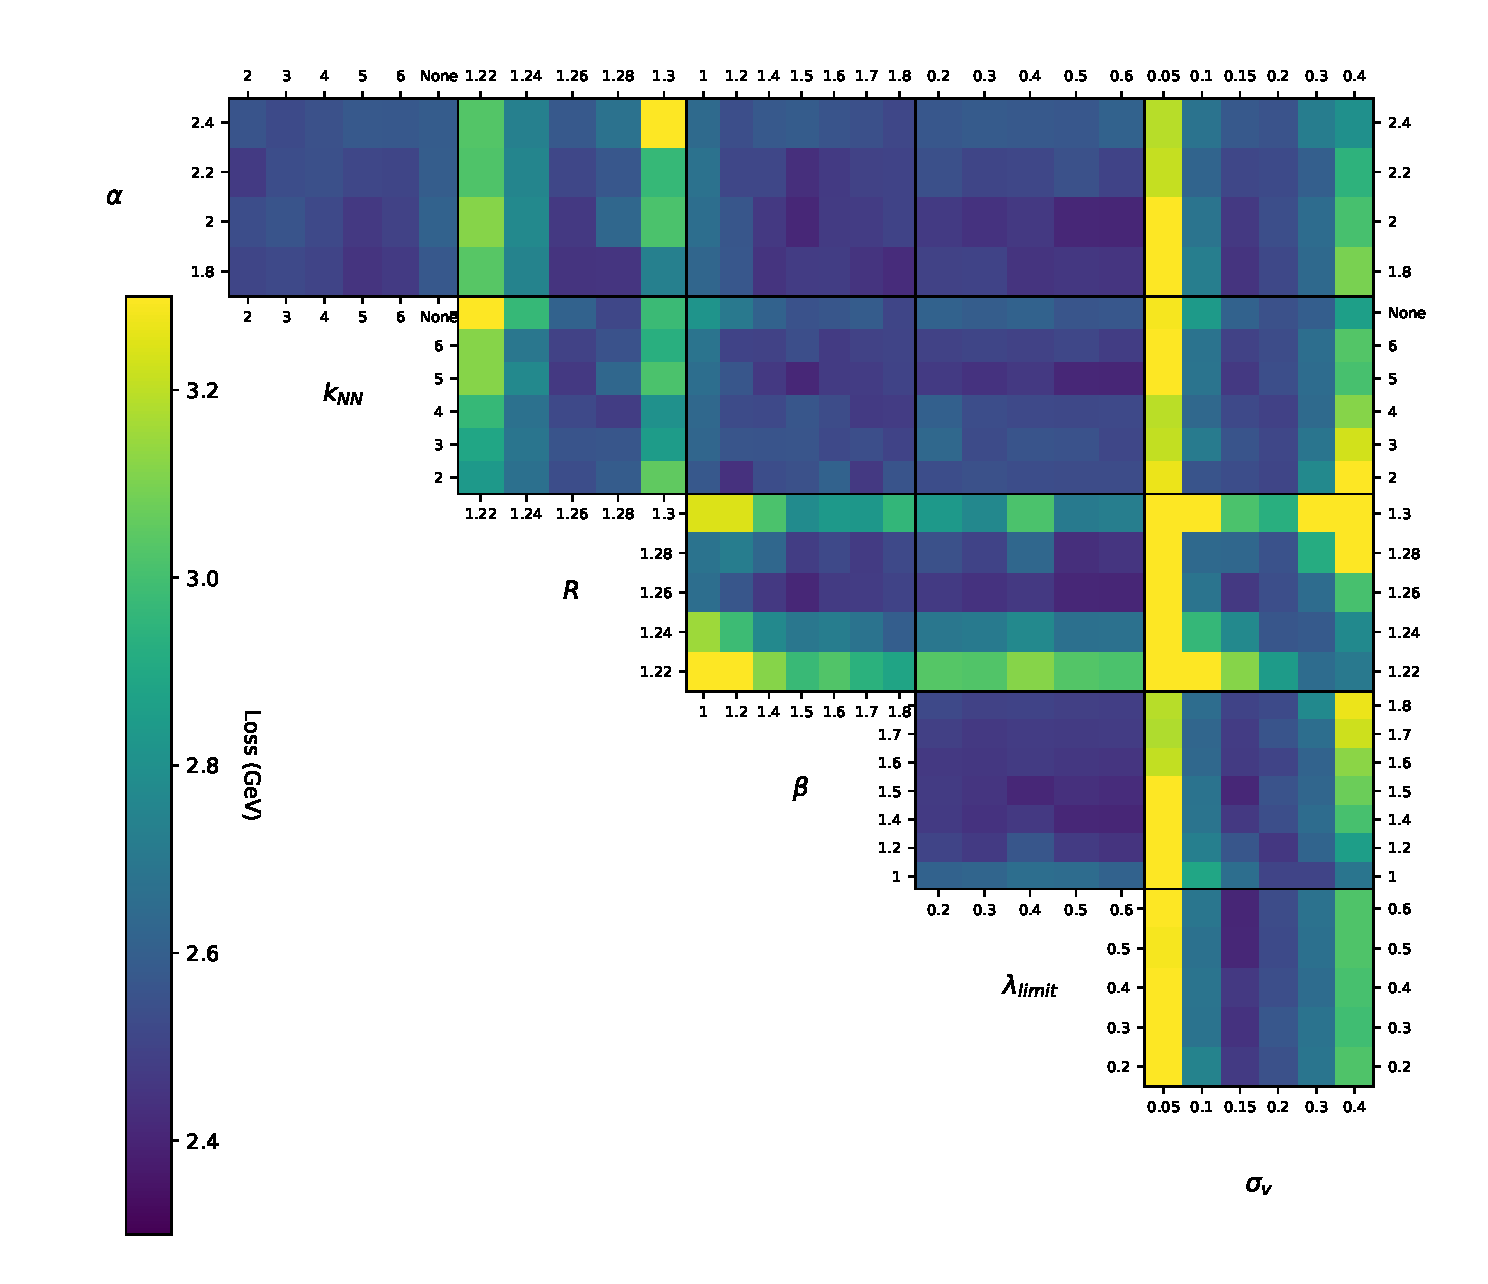
\includegraphics[width=1\textwidth]{graphics/trangle_scan_complete}
            \caption{There are 6 free parameters in \spectral{} clustering.
                Here, the ``Loss'', as described in Eq.~(\ref{eqn:loss}), is shown for reasonable  parameter ranges chosen
                either by convention (e.g., \(\alpha\) is typically \(1\) or \(2\))
                or according to physical scales (e.g., $\sigma_v$ is of order \(0.1\)).
             }\label{fig:scan_spectral}
    \end{figure}    


    \subsection{Particle data}\label{sec:particle_data}

To evaluate the behaviour of the spectral clustering method four datasets are used\footnote{The first two uses a 2-Higgs Doublet Model (2HDM) setup as described in Ref.~\cite{Chakraborty:2020vwj} while the last two are purely Standard Model (SM) processes. Notice that all unstable objects are rather narrow, including the Beyond the SM (BSM) Higgs states \cite{Moretti:1994ds,Djouadi:1995gv}, so that we have neglected interference effects with their irreducible backgrounds.}, all produced for the Large Hadron Collider (LHC).

    \begin{enumerate}
        \item 
    \underbar{Light Higgs} A SM-like Higgs boson with a mass \(125\) GeV decays into two light Higgs states with mass  \(40\) GeV,
    which in turn decay to \beau{}\bbar{} quark pairs.
    That is, the process is \(p p \rightarrow H_{125\,\text{GeV}} \rightarrow h_{40\,\text{GeV}} h_{40\,\text{GeV}} \rightarrow \beau \bbar \beau \bbar\), simulated at Leading Order (LO).

\item \underbar{Heavy Higgs}  A heavy Higgs boson with a mass \(500\) GeV decays into two SM-like Higgs states with mass  \(125\) GeV,
    which in turn decay to \beau{}\bbar{} quark pairs.
    That is, the process is \(p p \rightarrow H_{500\,\text{GeV}} \rightarrow h_{125\,\text{GeV}} h_{125\,\text{GeV}} \rightarrow \beau \bbar \beau \bbar\), simulated at LO.

\item \underbar{Top}  A $t\bar t$ pair decays semileptonically, i.e., where one \(W^\pm\) decays to a pair of quark jets $jj$ and the other into a lepton-neutrino pair $\ell\nu_\ell$ ($\ell=e,\mu$).
        That is, the process is \( p p \rightarrow t \bar{t} \rightarrow b\bar b W^+  W^-\to b\bar b jj \ell\nu_\ell\), simulated at LO. (Note that, here, $m_t=172.6$ GeV and $m_{W}=80.4$ GeV.)
        
    \item \underbar{3-jets}  For the purpose of checking {IR safety}, we have used three-jet events,         this being a rather simple configuration where IR singularities could be observed. 
        That is, the process is $pp\to jjj$, simulated at both LO and Next-to-LO (NLO). 



    \end{enumerate}

    Using MadGraph~\cite{Alwall:2011uj} to generate the partonic process and Pythia~\cite{Sjostrand:2014zea} to shower, ${\cal O}(10^5)$ of each of these processes are generated.
    A full detector simulation is not used; instead, cuts on the particles are imposed to approximate detector resolution, as detailed below. 
    
    The Center-of-Mass (CM) energy used is \(\sqrt{s}=13 \) TeV.

    Each event also contains (hard) Initial State Radiation (ISR) and soft QCD dynamics from beam remnants, i.e., the Soft Underlying Event (SUE).
    There is no pileup or multiparton interactions in the datasets.

    Each of these datasets requires different cuts, both at the particle level, to simulate detector coverage, and at the jet level, to select the best reconstructed events.
    The cuts on each dataset are as follows.
    \begin{enumerate}
        \item The reconstructed particles are required to have
            rapidity \(|\eta|< 2.5\) and (transverse momentum \(p_T > 0.5\) GeV.
            These cuts are likely to remove the majority of the radiation from beam remnants
            and reduce the radiation from ISR.
            The $b$-jets are required to have \(p_T > 15\) GeV, which is possibly lower than is realistic \cite{Chakraborty:2020vwj},
            but it leaves a larger number of events to compare the behaviour of jet clustering algorithms.

        \item  The reconstructed particles are required to have
             \(|\eta|< 2.5\) and \(p_T > 0.5\) GeV.
            The $b$-jets are required to have \(p_T > 30\) GeV, which is realistic for efficient $b$-tagging performance and further reduces ISR and the SUE.
            
        \item The reconstructed particles are required to have
             \(|\eta|< 2.5\) and \(p_T > 0.5\) GeV.
            The event is required to have  \(p_{T}^{\text{miss}} > 50\) GeV,
            where \(p_{T, \text{miss}}\) is the missing transverse momentum due to 
            the neutrino.
            The lepton in the event must have  \(|\eta|< 2.4\).
            If the lepton  is a muon then its \(p_T\) must be \(>  55\) GeV.
            If the lepton  is an electron and it is isolated (as defined in~\cite{Sirunyan:2018fpa}) then its \(p_T\) must be \(> 55\) GeV, if it is not isolated then \(p_T > 120\) GeV.
            The reconstructed jets must have \(p_T > 30\) and \(|\eta|< 2.4\).
            Finally, the lepton must be separated from the closest jet by at least
            \(\sqrt{\Delta\eta^2 + \Delta \phi^2} > 0.4\) or
            \(p_{T}^{\text{relative}} > 40\) GeV.
            These cuts are copied from~\cite{Sirunyan:2019rfa}.
        \item The only restriction on the particles is that the rapidity must be \(< 2.5\).
            There are no cuts on the jets. While unrealistic, since 
            issues of IR safety are emphasised at low \(p_T\),  to highlight this we abandon all \(p_T\) cuts.

    \end{enumerate}


    The Higgs boson cascade datasets have the desirable property of creating \bthing{jets} with different kinematics: while in case 1 we may expect some slim  jets (as on average they are rather stationary, because of the small mass difference between $H_{125\,{\rm GeV}}$ and $H_{40\,{\rm GeV}}$)
in case 2 we may see mainly fat jets (owing to the boost provided by the large mass difference between $H_{500\,{\rm GeV}}$ and $H_{125\,{\rm GeV}}$).
Mass reconstruction requirements for the \underbar{Light Higgs} and \underbar{Heavy Higgs} follow the same logic.
In order to reconstruct a Higgs decaying directly to a pair of \bthing{quarks}, we require a separate jet tagged by each \bthing{quark}, that is, two jets are required, each tagged by a \bthing{quark} from that Higgs.
To reconstruct a Higgs that decays to a pair of child Higgs particles,
we require both child Higgs bosons have been reconstructed,
that is, all four \bthing{jets} are found.
In the case of the \underbar{Top} events
three masses can be reconstructed from jets, the hadronic \(W\),
the hadronic top and the leptonic top.
The hadronic \(W\) is reconstructed if both of the quarks it decayed to have tagged jets; they are permitted to tag the same jet, so the hadronic \(W\) can be reconstructed from one or two jets.
The hadronic top is reconstructed if the hadronic top is reconstructed and the \bthing{quark} from the hadronic top has tagged a jet, so the correct \bthing{jet} is required in addition to the requirements on the \(W\).
The leptonic top is reconstructed if the \bthing{quark} from the top decay tags a jet, and the missing momentum calculation which reconstructs the leptonic \(W\) yields a real mass.
If the missing mass calculation for the mass of the leptonic \(W\) yields two real masses, the one closes to the \(W\) mass is selected.

We now proceed to compare spectral to anti-$k_T$ clustering and we start from testing IR safety of the former, while this is a well-known feature of the latter. We will then move on to study Higgs boson and top quark events.


\subsection{Determining IR safety}\label{sec:IRmethod}
    It would be possible to demonstrate IR safety analytically, however,
    as the environment required for clustering on MC data is already set up,
    it is more efficient for this study to prove IR safety with such data.
    This can be done by showing that an IR sensitive variable, for example, the jet mass spectrum,
    is stable between a LO dataset with no IR singularities and a NLO
    one which will instead contain IR singularities.

    Showing the jet mass spectrum at LO and NLO for a particular configuration,
    that is, a particular selection of clustering parameters,
    would allow a comparison that would highlight any differences caused by IR sensitivity.
    This will be done for illustrative purposes,
    however, even an IR unsafe algorithm, such as the iterative cone one~\cite{Cacciari:2008gp},
     has some configurations for which these singularities are avoided.

    To provide a more global view, a scan of parameter configurations must be compared.
    Thus, for an unsafe algorithm (such as the iterative cone) the unsafe configuration
    will be found.
    It would be cumbersome to compare all these jet mass spectrum by eye, however.
    Instead, we introduce a summary statistic representing the divergence between two distributions,
    the Jensen-Shannon score~\cite{Lin:1991zzm}.

    The Jensen-Shannon score is a value computed between two distributions that increases in magnitude the more these distributions differ.
    It is a symmetrised variant of the Kullback-Leibler divergence~\cite{Lin:1991zzm}.
    The Kullback-Leibler divergence between probability densities \(p\) and \(q\) can be written as
    \begin{equation}
    D_\text{KL} (p | q) = \int^{\infty}_{-\infty} p(x) \log\left(\frac{p(x)}{q(x)}\right) dx,
\end{equation}
    from which the Jensen-Shannon divergence can be written as
    \begin{equation}
    D_\text{JS}(p, q) = \frac{1}{2}D\left(p | \frac{1}{2}(p + q)\right) + \frac{1}{2}D\left(q | \frac{1}{2}(p + q)\right).
\end{equation}
    Here, \(D_\text{JS}\) treats \(p\) and \(q\) symmetrically and will grow as they become more different.
    The spectrum of Jensen-Shannon scores will be plotted for a known IR safe clustering algorithm, \antikt{},
    a known unsafe clustering algorithm, iterative cone, and the \spectral{} algorithm.
    If the Jensen-Shannon scores for \spectral{} are consistently small,
    then it is IR safe.

